\documentclass[12pt,a4paper]{article}

\usepackage{amsfonts}
\usepackage{amssymb}
\usepackage{amsmath}
\usepackage{amsthm}
\usepackage{enumerate}

\usepackage[utf8]{inputenc}
\usepackage{csquotes}
\usepackage{polski}
\usepackage[utf8]{inputenc} 
\usepackage[T1]{fontenc}
%\usepackage{indentfirst}
\usepackage{ wasysym }
\usepackage{hyperref}

\usepackage{tikz}
\usetikzlibrary{arrows}

\frenchspacing

%\renewcommand{\arraystretch}{3.0}
%\renewcommand{\thefootnote}{\fnsymbol{footnote}}


\newcommand{\norm}[1]{\left\lVert#1\right\rVert}

% Pisanie za każdym razem \mathbb{R} jest zbyt długie, teraz wystarczy \RR.
\newcommand{\RR}{\mathbb{R}}
% tak samo \overrightarrow
\newcommand{\V}[1]{\overrightarrow{#1}}
\newcommand{\Pair}[2]{\left<#1,#2\right>}
\renewcommand{\qed}{$\square$}

% Definicja stylów:
\theoremstyle{plain}
\newtheorem{tw}{Twierdzenie}[section]
\theoremstyle{definition}
\newtheorem{ft}{Fakt}[section]
\theoremstyle{definition}
\newtheorem{df}{Definicja}[section]
\theoremstyle{definition}
\newtheorem*{nt}{Notacja}
\theoremstyle{definition}
\newtheorem*{dd}{Dowód}
\theoremstyle{definition}
\newtheorem*{lem}{Lemat}
\theoremstyle{definition}
\newtheorem*{prz}{Przykład}
\theoremstyle{definition}
\newtheorem*{przy}{Przykłady}
\theoremstyle{definition}
\newtheorem*{uw}{Uwaga}
\theoremstyle{definition}
\newtheorem*{wn}{Wnioski}

\begin{document}
\section{Przekształcenia liniowe} 
\begin{df}
    Przekształceniem liniowym (homomorfizmem) przestrzeni liniowych $V \text{ i } W$ nazywamy odwzorowanie $F: V \rightarrow W$ t. że
    \begin{enumerate}[{(}1{)}]
        \item $\forall v, v' \in V \quad F(v+v') = F(v) = F(v')$ (addytywność) 
        \item $\forall v \in V \ \forall \alpha \in K \quad F(\alpha v) = \alpha F(v)$ (jednorodność)
    \end{enumerate}
\end{df}

\begin{przy}
    \hfill
    \begin{enumerate}[{(}1{)}]
        \item $F: \RR^n \rightarrow \RR, \quad F \left( \begin{pmatrix} x_1 \\ \vdots \\ x_n \end{pmatrix}\right) = \alpha_1 x_1 + \dots + \alpha_n x_n \text{, ustalone } \alpha_i \in \RR$ 
        \item $F: \RR^n \rightarrow \RR^m  \quad F \left( \begin{pmatrix} x_1 \\ \vdots \\ x_n \end{pmatrix}\right) = \begin{pmatrix} \alpha_{1,1}x_1 + \dots + \alpha_{1,n} x_n\\ \vdots \\ \alpha_{m,1}x_1 + \dots + \alpha_{m,n} x_n \end{pmatrix}$
        \item $F: K^n \rightarrow K, \quad F \left( \begin{pmatrix} x_1 \\ \vdots \\ x_n \end{pmatrix}\right) = \alpha_1 x_1 + \dots + \alpha_n x_n \text{, ustalone } \alpha_i \in K$ 
        \item $F: K^n \rightarrow K^m  \quad F \left( \begin{pmatrix} x_1 \\ \vdots \\ x_n \end{pmatrix}\right) = \begin{pmatrix} \alpha_{1,1}x_1 + \dots + \alpha_{1,n} x_n\\ \vdots \\ \alpha_{m,1}x_1 + \dots + \alpha_{m,n} x_n \end{pmatrix}$
        \item $F : C'(\RR) \rightarrow C(\RR) \quad F(f) = f'$ 
        \item $F: C(\RR) \rightarrow C(\RR) \quad F(f) = \int\limits_0^x \ f(y) dy$ 
        \item $F: C(\RR) \rightarrow \RR \quad F(f) = \int\limits_a^b \ f(x) dx$ 
        \item $F: \RR [x] \rightarrow \RR[x] \quad F(P)(x) = xP(x)$
        \item $F: C(\RR) \rightarrow \RR \quad F(f) =f(7)$
        \item $L: F(\mathbb{N},\RR)  $ \\ %pierdolona strzałka
        $L((a_1,a_2,\dots)) = (a_2,a_3,a_4,\dots)$ \\
        $R((a_1,a_2,\dots)) = (0,a_1,a_2,\dots)$ 
    \end{enumerate}
\end{przy}
\begin{ft} \hfill 
    \\
    $F: U \rightarrow V $ i $G: V \rightarrow W$ liniowe, to $G \circ F: U \rightarrow W $ liniowe. 
\end{ft}

\begin{dd}
    $(G \circ F)(u+u') = G(F(u+u')) = G(F(u) + F(u')) = G(F(u)) + G(F(u')) = (G \circ F)(u) + (G \circ F)(u') $ (analogicznie jednorodność)
\end{dd}

\begin{df} \hfill \\
    $F: V \rightarrow W $ p. lin \\
    \underline{Obrazem} F nazywamy \\
    $Im F = \{ F(v): v \in V\}$ \\
    \underline{Jądrem} F nazywamy \\
    $ker(F) = \{v: F(v) = 0\}$ \\
\end{df} 
\begin{ft} \hfill 
    \begin{enumerate}[{(}1{)}]
        \item $Im F < W$
        \item $kerF < V$
    \end{enumerate}
\end{ft}

\begin{dd} 
    ~\\
    $w,w' \in Im F \quad w=F(v), w'=F(v')$ \\
    $w+w' = F(v) + F(v') = F(v+v') \Rightarrow w+w' \in ImF$ (podobnie dla mnożenia) \\
    $v,v' \in ker F \quad F(v) = F(v') = 0$ \\
    $F(v+v') = F(v) + F(v') = 0 + 0 = 0 \Rightarrow v+v' \in ker F$ (podobnie dla mnożenia)
    \qed
\end{dd}

\begin{uw}
    $F: V \rightarrow W $ liniowe
    $F(0) = $ %AHA
    zatem $\{0\} \subseteq ker F$.
\end{uw}

\begin{ft} 
    ~\\
    $F: V \rightarrow W $ p. lin jest różnowartościowe \\
    $ \hspace*{30mm} \Updownarrow \\
        \hspace*{20mm} ker F = \{ 0 \}
    $
\end{ft}

\begin{dd} \hfill
    \begin{itemize}
        \item[$(\Uparrow)$] $F(v) = F(v') \\ 
            F(v)-F(v') = 0 \\
            F(v-v') = 0 \\
            ker F \ni v-v' = 0 \\
            v = v' 
        $ \qed
        \item[$(\Downarrow)$] oczywiste
    \end{itemize}
\end{dd}

\begin{tw}[o indeksie]
    ~\\
    $F: V \rightarrow W $ liniowe, to $dimker F + dimIm F = dim V$
\end{tw}
\newpage
\begin{dd}
    ~\\
    $ker F < V,\  Im F < W$ \\
    \begin{minipage}[c]{0.5\textwidth}
        $B$ - bzaza $ker F$ \\
        $ B \cup B' $ - baza $V$
    \end{minipage}%
    \begin{minipage}[c]{0.5\textwidth}
        $B = \{b_i\}_{i \in I}$ \\
        $B' = \{b'_i\}_{i \in J}$ \\
        $I \cap J = \emptyset $
    \end{minipage}
    %też trzeba wstawić jakiś gówniak, w sensie przerwę coś się dzieje i sie nie pojawia xD 
    bazą $Im F$ jest $\{F(b'_i)\}_{i \in J}$ \\
    Będziemy teraz udowadniać, że to rzeczywiście jest baza\\
    $w \in Im F$ \\
    %piękny obrazek
	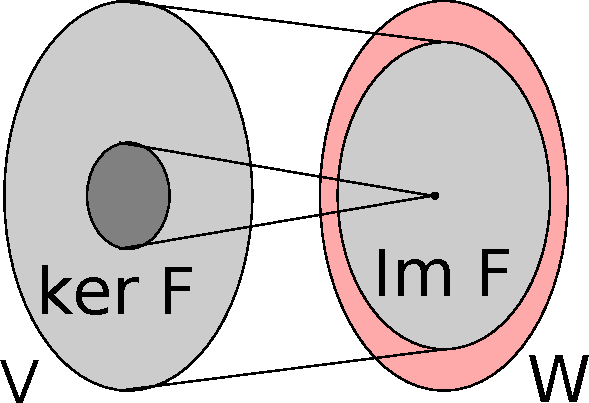
\includegraphics[width=5cm]{wyklad3_obrazek} \\ % konwertowanie:

    $w = F(v) = F(\sum\limits_{i \in I'} \alpha_i b_i + \sum\limits_{i \in J'} \alpha'_i b'_i) = \sum\alpha_i b_i + \sum\alpha'_i b'_i = \sum\alpha'_i b'_i $\\
    $(|I'|, |J'|<\infty \quad I'\subset I, J'\subset J)$\\
    więc $\{F(b'_i)\}_{i \in J} $ generuje $ImF$ \\
    $\sum\limits_{i\in J} \alpha'_i F(b_i') = 0$\\
    $\qquad \rotatebox{90}{$\,=$}$\\%nie umiem zrobić odstępu :(
    $F(\sum \alpha'_i b_i') \quad $więc $ \sum \alpha'_i b_i' \in imF$\\
    $\sum \alpha'_i b_i' =\alpha_i b_i$ \quad kombinacja liniowa bazy $kerF$\\
    $B\cup B'$ jest bazą V więc $\alpha_i' = \alpha_i = 0$ \quad \qed
     % dopisać resztę linijki 
    %wniosek generuj Im i dowód lnz
\end{dd} 

\begin{prz}
    $ V = \{ P \in \RR_4[x] : P'(0) + P(0) = P(1) = 0 \}$ 
    \begin{itemize}
        \item V jest p. liniową
        \item Obliczyć $dim V$
    \end{itemize}
    $ F : \RR_4[x] \rightarrow \RR^4 
        \qquad F(P) = \begin{pmatrix} P'(0) + P(0) \\ P(1) \end{pmatrix} $ \quad $F$ jest liniowe \\
    $V = ker F$, czyli $V < \RR_4[x]$
    $dim V = dimker F = dim\RR_4 [x] = dimImF$ %skrabione znaki równa się \\
    $F(1) = \begin{pmatrix} 1 \\ 1 \end{pmatrix} \in Im F$ \\
    $F(x^2) = \begin{pmatrix} 0 \\ 1 \end{pmatrix} \in Im F$
    $Lin \left\{ \begin{pmatrix} 0 \\ 1 \end{pmatrix} \begin{pmatrix} 1 \\ 1 \end{pmatrix} \right\} < Im F < \RR^2 $, czyli
    $Im F = \RR^2$ \\%+ popierdolone równa się xD
    $dimV = dim\RR[x] - dimImF = 5 - 2 = 3$
\end{prz}

\begin{df} 
    Przekształcenie liniowe $F: V \rightarrow W $ nazywamy odwracalnym $\Leftrightarrow$ istnieje $G: W \rightarrow V$ liniowe t. że $F \circ G - id_W, G \circ F = id_V.$ Przekształcenie odwrotne (o ile istnieje) jest jedyne i oznaczamy je $F^{-1}$. \footnote{$(F \circ G)(v) = F(G(v))$}
\end{df}

\begin{ft} $F: V \rightarrow W $, liniowe, $dim V = dimW < \infty$. Wówczas NWSR:
    \begin{enumerate}[{(}1{)}]
        \item $F$ różnowartościowe (tzn. $kerF = \{0\}$)
        \item $F$ jest "na" (tzn. $Im F = W$)
        \item $F$ jest bijekcją
    \end{enumerate}
\end{ft}

\begin{dd} 
    ~\\
    $dimker F + dimIm F = dim V = dim W$
    \begin{itemize}
        \item[$(1) \Rightarrow (2)$] $
            dimker F = 0, \qquad Im F < W \\
            dimIm F = dim W \\ 
            Im F = W$
        \item[$(2) \Rightarrow (3)$]
            $
            dimImF = dimW \\
            dimkerF = 0 \\ 
            kerF = \{0\} \\
            F
            $ różnowartościowa + "na"
        \item[$(3) \Rightarrow (1)$] oczywiste
    \end{itemize} 
\end{dd}

\begin{df} 
    Niech $B = (b_1,\dots,b_n) $ będzie bazą przestrzeni liniowej V. Wówczas \underline{współrzędnymi} wektora $v \in V$ w bazie B nazywamy: 
        $$ [v]_B = \begin{pmatrix} \alpha_1 \\ \vdots \\ \alpha_n \end{pmatrix} \quad \alpha_i \in K$$ \\
        gdzie $ v = \alpha_1 b_1 + \dots + \alpha_n b_n$.
\end{df}

\begin{df} 
    $ 
        F: V \rightarrow W \text{p. liniowa nad K} \\
        B = (b_1,\dots,b_n) \text{ - baza V} \\
        C = (c_1, \dots,c_m) \text{ - baza W} \\
    $
    Wówczas macierz \\
        $$m^B_C (F) = ([F(b_1)]_C,\dots,[F(b_n)]_C)$$ nazywamy \underline{macierzą przekształceń $F$} w bazach $B$ i $C$. 
    $$ A = \begin{pmatrix} a_{11} \ a_{12} \ \dots \ a_{1n} \\
                           a_{21} \ a_{22} \ \dots \ a_{2n} \\
                                   \        \vdots \  \\
                           a_{m1} \ a_{m2} \ \dots \ a_{mn}
    \end{pmatrix} \quad A \in M_{m \times n} (K)$$
\end{df}
\noindent 
\underline{Dodawanie macierzy} \\
$ 
  A = (a_{ij}) \\
  A' =(a'_{ij}) \\ 
  B = A + A' = (b_{ij}), \text{gdzie} b_{ij} = a_{ij} + a'_{ij}
$ \\
\underline{Mnożenie macierzy przez skalar} \\ 
$ 
    t \in K, (a_{ij}) = A \in M_{m \times n}(K) \\
    tA = B = (b_{ij}) \quad b_{ij} \overset{\mathrm{def}}{=} t a_{ij}
$ \\
\underline{Mnożenie macierzy} \\ 
$
    A = (a_{ij}) \in M_{m \times n} \\
    B = (b_{ij}) \in M_{n \times l} \\ 
    C = A \cdot B = (c_{ij}) \in M_{m \times l} \\
    c_{ij} \overset{\mathrm{def}}{=} \sum\limits_{k=1}^n a_{ik}b_{kj}
$
\begin{ft}
    Mnożenie \\
    $A', A \in M_{k \times l} (K) \hspace{0.5cm} B', B \in M_{l \times m} (K) \hspace{0.5cm} C \in M_{m \times n} (K)$
    \begin{enumerate}[{(}1{)}]
        \item $ (A \cdot B) \cdot C = A \cdot (B \cdot C)$
        \item $ (A + A') \cdot B = A \cdot B + A' \cdot B \\
            A \cdot (B + B') = A \cdot B + A \cdot B' $
        \item $ I_k \cdot A = A  \cdot I_l = A  \hspace{1cm} \text{gdzie } I_k = \begin{pmatrix} 
                1 \ ~~ \ 0 \\ ~~ \ \ddots \ ~~ \\ 0 \ ~~ \ 1
            \end{pmatrix} $
    \end{enumerate}
\end{ft}

\begin{ft}
    Niech \\ $ F: V \rightarrow W $ będzie przekształeceniem liniowym.\\
    $ B = (b_1, \ldots , b_n) \text{ - bazą } V \\
      C = (c_1, \ldots , c_n) \text{ - bazą } W $ \\
    Wówczas:
    $$ [F(v)]_C = m^B_C(F) \cdot [v]_B \text{ ,gdzie } v \in V$$
\end{ft}

\begin{wn}
    $ id: V \rightarrow V,\quad B, C \text{ - bazy } V$
    $$ [v]_c = m^B_C(id) \cdot [v]_B $$
    gdzie $ m^B_C(id) = ( [b_1]_C, \ldots , [b_n]_C)$
\end{wn}

\begin{ft}
    Niech \\ $ F: U \rightarrow V, G: V \rightarrow W $ będą przekształceniami liniowymi.\\
  $ B \text{ - bazą } U\\
    C \text{ - bazą } V\\
    D \text{ - bazą } W\\ $
Wtedy: $m^B_D(G \circ F) = m^C_D(G) m^B_C(F)$
\end{ft}
\begin{wn}
$ id: V \rightarrow V,\quad B, C \text{ - bazy } V$
    Wtedy: $$ m^B_B(F) = m^C_B(id) \cdot m^C_C(F) \cdot m^B_C(id)$$

\end{wn}
\end{document}
